%%%%%%%%%%%%%%%%%%%%%%%%%%%%%%
%% intro.tex
%%%%%%%%%%%%%%%%%%%%%%%%%%%%%%

The idea of quantum computer dates back at least to Feynman~\cite{Feynman1982Simulating}, who speculated a possibility for exploiting the computational power that Nature allows. The idea raises a deep question. The computation is a manipulation of symbols and numbers according to our logical system. If we can simulate the time evolution of Nature in a controllable and mechanical way, then it is unavoidable to conclude that the present Nature is really computing the future, and that the way she does is essentially the same as our arithmetic. If we cannot simulate what she does, then it means there is a fundamental difference between the time evolution and its artificial simulation by our logic and numbers. Either conclusion must have profound consequences.



An important problem in proving the possibility of a quantum computer is how to suppress decoherence. Shor discovered a scheme in which as long as elementary operations have a low enough error rate one can perform an arbitrarily long computation~\cite{Shor1996Fault-tolerant}. He showed there is a positive constant $\delta$ such that any ideal computation can be simulated by faulty elementary operations if they are close to ideal ones up to precision $\delta$; the scheme effectively reduces the error rate. Thus, the problem of decoherence is solved at least theoretically. 



Kitaev proposed yet different scheme, called topological quantum computation, in which elementary operations are physically protected and hence are ideal for all practical purposes~\cite{Kitaev2003Fault-tolerant}. He pointed out that there is a naturally protected subspace in topologically ordered systems in two spatial dimensions. The subspace is accessible by braiding excitations, so-called anyons. As long as the anyons are geometrically well separated at any time step of the computation, the subspace remains decoherence-free. A classical analog is easy to understand. In a magnetic storage medium a bit is encoded into one of two polarizations of little ferromagnets. Each little ferromagnet consists of billions or more electrons whose spins are aligned together. An electron spin may be flipped by some error, but it is energetically unfavorable. Many errors require high energy, and it is very unlikely that the average magnetization would change the sign. The main idea of the encoding quantum information in the topologically ordered system is similar. The information is carried not by local degrees of freedom, but by collective degrees of freedom, where local errors are suppressed by natural means.



A requirement for a system to be useful for the topological quantum computation is that the system must have eigenstates of the same energy that are locally indistinguishable. The states only look different when one has a full description of them; the local reduced density matrices are identical. This property has no classical analog. Systems whose ground states are locally indistinguishable are already found. The fractional quantum Hall systems with a filling fraction $\nu = p/q$ have $q$ degenerate ground states that are locally indistinguishable~\cite{Haldane1985MagneticTranslation,WenNiu1990GroundState}. The local indistinguishability accompanied by a finite energy gap above the degenerate ground states, has a significant consequence that the degeneracy does not split in the thermodynamic limit, even under general local perturbations~\cite{WenNiu1990GroundState,Kitaev2003Fault-tolerant,BravyiHastingsMichalakis2010stability}.
This intrinsic stability underlies the idea to build a quantum computer on topologically ordered systems~\cite{
DennisKitaevLandahlEtAl2002Topological,
JiangBrennenGorshkovEtAl2008Anyonic, 
SarmaFreedmanNayak2005Topologically}.



However, a closer analysis reveals that the topologically ordered system is vulnerable to thermal fluctuations~\cite{AlickiFannesHorodecki2009thermalization}. The collective degrees of freedom are well protected as long as the anyons are far separated, but the thermal fluctuations cause the anyons to propagate randomly throughout the system. The random motions are not a priori suppressed by, for example, energetics. Anyonic systems do not function as protected media as the magnetic media do for classical information storage. That any topologically ordered system has a naturally protected subspace is not entirely true.



We need to separate the problem for further concrete discussions. A computer is loosely divided into two parts: reliable storage and fault-tolerant processing of information. The division is not too fundamental since the storage may require some sort of ancillary information processing, and vice versa. It is a convenient division for the sake of analysis. The storage problem for quantum information concerns a possibility of a quantum analog of classical hard disk drive, which we call a \emph{self-correcting quantum memory}. One asks if there is a system where a subspace is maintained coherently as collective phenomena~\cite{DennisKitaevLandahlEtAl2002Topological,Bacon2006Operator}. The processing problem concerns a wise choice of an elementary operation set and its implementation, and is thus contingent upon the storage scheme. In this thesis we focus on the storage problem.


The result of the present thesis can be summarized as follows. We find a spin model on a three-dimensional cubic lattice, whose excitations are immobile and point-like. Under any perturbation the excitations do not acquire a kinetic term --- any hopping amplitude  vanishes exactly. Moreover, the ground-state subspace is degenerate, exactly in the thermodynamic limit, and no local order parameter can be defined. These properties do not fit into intuitive pictures people had about the topological order. The reason why it is unconventional will be explained below. Given the model, we devise a scheme to use it as quantum memory and compute the storage time. We prove a rigorous lower bound on the storage time that grows with system size up to an optimal value $T_{mem} = e^{\Omega(\beta^2)}$ where $\beta$ is an inverse temperature of a heat reservoir. It should contrast with a conjectured storage time $e^{O(\beta)}$ of any two-dimensional topologically ordered system.


We briefly review how the concept of topological order has emerged, and discuss our results.


\section{Topological order}

The quantum Hall effects are phenomena in which the transversal conductance becomes a locally constant function (plateau) for ranges of perpendicular magnetic field strength. In the integer quantum Hall effect, as the magnetic field is increased, the Hall conductance develops plateaus at quantized values of $n e^2/h$ in the vicinity of field $B = \rho_0 hc/ne$ where $n$ is a small positive integer and $\rho_0$ is the electron number density~\cite{KlitzingDordaPepper1980IQHE}. The quantization is very accurate and universal. The measured conductances from various experiments all agree with one another within a relative error less than a part in a million~\cite{PrangeGirvin1990HallEffect}. The agreement is so remarkable because different experiments do not fine-tune every aspect of experimental setups up to precision $10^{-6}$. Due to its simple reproducibility and high accuracy, the integer quantum Hall effect is now used to define an international standard of resistance~\cite{SI2008}.

The exact quantization can be explained by Laughlin's argument~\cite{Laughlin1981QHE}, refined by Halperin~\cite{Halperin1982QHE}. They consider an adiabatic insertion of magnetic flux near the boundary of the Hall sample. They conclude that the Hall conductance is quantized because extended (delocalized) electronic states near the sample edge whose energies are far from Fermi level are only responsible for the conductance. Thouless {\em et al.}~\cite{TKNN1982} showed that those extended states actually define a topological vector bundle whose invariant, now called TKNN invariant or Chern number, is directly related to the quantized Hall conductance.

The awe of the quantum Hall effects does not end there. Soon after the discovery of the integer quantum Hall effects, another kind of quantization was measured --- the fractional quantum Hall effects~\cite{TsuiStoermerGossard1982FQHE,Laughlin1983FQHE}. The transversal conductance displays many plateaus at fractional multiples of $e^2/h$, not only at integral multiples of $e^2/h$.
An interesting feature is the structure of the ground-state subspace. There are $q$-fold degenerate ground states for a fractional quantum Hall system of filling fraction $\nu = p/q$ defined on a torus, where $p$ and $q$ are co-prime integers~\cite{NiuThoulessWu1985Topological,Haldane1985MagneticTranslation}. By taking a detour through an effective theory, the degeneracy is argued to be a function of topology~\cite{WenNiu1990GroundState}. More specifically, if a fractional quantum Hall Hamiltonian at $\nu = p/q$ is defined on a Riemann surface of genus $g$, the degeneracy is $q^g$.

It is much more interesting that quasi-particles of the fractional quantum Hall system are thought to be {\em anyons}~\cite{Wilczek1982Anyon}. They obey neither bosonic nor fermionic statistics under exchange. Rather, the wave function of two-anyon state may be transformed by a unitary operator if one anyon is transported around the other. It has been conjectured that the nonabelian case, where the unitary is not just a phase factor, could be realized in a fractional quantum Hall system at certain filling fractions $\nu = p/q$~\cite{WillettEtAl1987EvenFQHE,MooreRead1991Nonabelions}. Unfortunately, the nonabelian statistics has not been verified experimentally.

Meanwhile, the concept of topological order had emerged. It was introduced as an abstract notion to describe the fractional quantum Hall systems and spin liquid states~\cite{WenWilczekZee1989Chiral}. A gapped system is generally said to be topologically ordered if the ground-state subspace is degenerate but no symmetry is spontaneously broken, and the degeneracy is robust under any perturbation in the thermodynamic limit~\cite{Wen1991SpinLiquid,ReadSachdev1991LargeN}. Also, the degeneracy as a function of physical space topology and the anyonic quasi-particle statistics are taken as defining characteristics of topological order~\cite{WenNiu1990GroundState,Kitaev2003Fault-tolerant,MooreRead1991Nonabelions}.

Another important yet different characteristic is topological entanglement entropy~\cite{KitaevPreskill2006Topological, LevinWen2006Detecting}. A ground-state wave function of a gapped Hamiltonian is believed to obey an area law. Namely, the von Neumann entropy $S(\rho)$ of the reduced density matrix $\rho$ for a disk region is bounded from above by a constant times the area of the boundary. In our two-dimensional situation, the area is the perimeter of the boundary, so $S(\rho) \le \alpha L$. The topological entanglement entropy is a negative constant correction to the area law; $S(\rho) = \alpha L -\gamma$. Remarkably, the $\gamma$ is insensitive to microscopic details and constant under deformation of the Hamiltonian as long as the deformation does not close the energy gap. This quantity is quite different in nature compared with other characteristics of topological order, since it is computed from a single wave function whereas the others are defined for Hamiltonians.

The topological order can be better understood by studying lattice gauge theories~\cite{Kogut1979LGT} and the toric code model~\cite{Kitaev2003Fault-tolerant}. One of the purposes to introduce lattice gauge theories is to contrast how our new model, called {\em cubic code}, is different from models in a conventional picture. The simplest possible lattice gauge theory is the Ising gauge theory due to Wegner~\cite{Wegner1971IsingGauge}. Ising gauge theory can be defined in any dimensions, but let us focus on the two-dimensional square lattice first. Later we will see a direct relation to the toric code model.


Consider the two-dimensional square lattice with a Ising variable (spin) $Z = \pm 1$ at each edge. For each vertex $v$, let $A(v)$ be an operator that flips four spins around $v$; $A(v) : \pm 1 \mapsto \mp 1$. $A(v)$ is called a {\em gauge transformation}. We can express it as an operator.
\[
 A(v) = X(N,v) X(W,v) X(S,v) X(E,v)
\]
where $X(N,v)$ means the matrix $\begin{pmatrix} 0 & 1 \\ 1 & 0 \end{pmatrix} \begin{matrix} \ket{+1} \\ \ket{-1} \end{matrix}$ 
acting on the north edge of the vertex $v$, and similarly for others.
We identify all states that related by the gauge transformations.
We look for a ``local'' Hamiltonian that is invariant under the action of $A(v)$.
Here, the locality may be ambiguous since we have identified states that differ by the gauge transformations
and formed a Hilbert space that is not a tensor product of local constituents.
However, the locality is still a proper notion with respect to the square lattice.


The gauge invariance allows restricted possibilities of terms in the Hamiltonian.
It is not hard to see that a term in the Hamiltonian must be a product of $Z$'s along a closed loop.
The simplest closed loop is a single plaquette. Thus, the simplest Hamiltonian would be given by the sum over all plaquettes $p$
\begin{equation}
 H = -J \sum_p B(p) = - J \sum_p Z(b,p) Z(r,p) Z(t,p) Z(l,p)
\label{eq:2D-Ising-gauge}
\end{equation}
where $J > 0$ and $B(p)$ is the product of four Ising variables on the bottom, right, top, and left of the plaquette $p$. It is important that the ground-state subspace does not spontaneously break any gauge symmetry. It is a general statement (Elitzur's theorem~\cite{Elitzur1975}) whose proof is not difficult~\cite{Kogut1979LGT,ChesiLossBravyiEtAl2010Thermodynamic}.


If $H$ is defined on a torus with periodic boundary conditions, there are four ground states that are not equivalent under the gauge transformations. This can be understood by visualizing configurations by loops. The configuration $C_0$ with all spins taking $+1$ values is a ground state of $H$. Any equivalent state under the gauge transformations is obtained by applying $A(v)$ at vertices. A single $A(v)$  flips four spins. Imagine connecting those flipped spins by straight lines --- they will form a loop. Applying more gauge transformations $A$ at various vertices, one adds more loops or deforms the loops. What is always true is that the loops are homologically trivial. Indeed, $A$ can be interpreted as a boundary operator in the cellular homology with $\ZZ/2$ coefficient acting on the dual 2-cells. What if we start with a configuration $C_1$ with all spins $+1$ except those $-1$ along a homologically nontrivial loop of the torus? Since $A$ does not alter the homology class of the configuration, we conclude that $C_0$ and $C_1$ cannot be equivalent under the action of $A$. Since there are 4 distinct homology classes of the torus including the trivial one $C_0$, the degeneracy is therefore 4. We emphasize that the homology classes are not locally distinguishable.

One can generalize the model so that it is defined on an arbitrary surface with a triangulation. The gauge transformations will be defined for each vertex, and the Hamiltonian will be a sum of all terms $B$, the product of Ising variables along the perimeter of elementary triangles. The homology description will be valid as well. The degeneracy is a function of homology of the surface.

Returning to the square lattice, we ask how an excited state looks like. It is described by unhappy terms $B(p) = -1$ in $H$. If we flip a spin from a ground state, then the two adjacent plaquette terms will become unhappy. If we flip two spins, say, one on the left and another on the right of a plaquette $p_0$, $B(p_0)$ will remain happy but those on the left plaquette and on the right will not. Generally, if we flip spins from a ground state such that flipped spins form a string on the dual lattice, then only two plaquette terms positioned at the end of the string will be unhappy. Those unsatisfied terms can be isolated at constant energy cost, and appear as the end points of the strings. If the string is extended to the infinity in one direction, there will be a single excitation. This is a topological excitation, in the sense that it cannot be created by a local operator, unlike a pair of nearby excitations. Note that the string that creates excitation has no gauge-invariant meaning. Applying $A(v)$ in the middle of an extended string will deform the string. The homological argument above shows that if two strings with the same end points differ by a homologically trivial cycle, the two strings describe exactly the same excited states.


The properties of the Ising gauge theory we have reviewed here
satisfy several criteria for topological order.
Its degeneracy is a function of topology, and no symmetry is spontaneously broken.
The four-dimensional ground space is stable under gauge-invariant perturbations.
Can we obtain a similar model without the gauge symmetry?
A prescription is to promote gauge transformations to be dynamical~\cite{Kitaev2003Fault-tolerant},
and take the Hilbert space as the tensor product of individual spins.
In other words, one adds gauge fixing terms to the Hamiltonian.
\begin{equation}
 H' = - J \sum_p B(p) - g \sum_v A(v)
\label{eq:H'}
\end{equation}
Since the Hamiltonian $H$ is constructed to be invariant under the gauge transformations, the new quantum Hamiltonian $H'$ is exactly solvable. The ground state is an equal-weight superposition of all equivalent spin configurations under the old gauge transformations. 
Our analysis on the absence of local order parameters and the degeneracy 
using the cellular homology is still valid. 
As the homology classes of spin configuration in the Ising gauge theory were not locally distinguished, 
the quantum ground states of $H'$ are not locally distinguished.
It follows that the degeneracy is not lifted under any local perturbations~\cite{BravyiHastingsMichalakis2010stability}.
Indeed, it is easily checked that the first order degenerate perturbation theory 
is vacuous because any local operator sandwiched between two ground states $\ket{a}$ and $\ket{b}$ 
is proportional to $\langle a | b \rangle$.

The gauge symmetry is not strictly imposed any more, but a particular gauge choice is energetically preferred.
Accordingly, there is one more type of excitations given by unsatisfied $A(v)$ terms, known as $e$-particles.
A violated $B(p)$-term is known as $m$-particle. 
Note that there is a duality between $A$ and $B$ terms. 
$A$ consists of Pauli $X = \sigma^x$ acting on a plaquette on the dual lattice, 
and $B$ consists of Pauli $Z = \sigma^z$ acting on a plaquette on the primary lattice. 
A pair of $m$-particles can be created from a ground state 
by applying ``spin flip'' operators $X$ along a string on the dual lattice.
A pair of $e$-particles can be created from a ground state by applying ``phase flip'' operators $Z$ along a string on the primary lattice. The $e$- and $m$-particles display mutual anyonic statistics. When one makes a complete circle around the other, the wave function acquires a phase factor $-1$. The topological entanglement entropy is nonzero~\cite{KitaevPreskill2006Topological, LevinWen2006Detecting}. We obtained an exactly solvable simple model with topological order, the {\em toric code}.


\section{String operators}

The string operators in the toric code deserve much attention. They are topological objects in that only the homological classes they represent matter. The fact that the strings are extended objects makes it clear how two particles at a distance may interact by braiding. The nontrivial braiding, in turn, implies a nontrivial ground-state subspace. The argument is basically the same as the proof of the degeneracy of the fractional quantum Hall system using magnetic translations~\cite{Haldane1985MagneticTranslation}.

The string picture seems to be correct for all two-dimensional topologically ordered systems. The robust degeneracy implies that there is no local observable that can distinguish different ground states; otherwise, perturbing the system with that local observable will lift the degeneracy. A minimal ``global'' operator whose support is not local would be a string operator stretched across the system. Another conceivable argument is as follows. Consider a region $R$ as large as possible on which no observable can resolve the ground-state subspace. If we assume translation invariance so we can unambiguously speak of thermodynamic limit, then a local operator is any operator with a bounded support. Hence, on a torus geometry, $R$ can be taken as the whole system minus two narrow strips, ensuring $R$ to be a contractible region. Since any operator in $R$ cannot resolve the ground-state subspace, some operator in the strips must be able to resolve it, which suggests the existence of string operators. As we will see in Chapter~\ref{chap:additive-codes}, the argument here can be made rigorous for a class of models. Also, there is an attempt to understand every possible model in two dimensions with the string picture~\cite{LevinWen2003Fermions,LevinWen2005String-net}.


What will happen if we go to three spatial dimensions? Consider a three-dimensional Ising gauge theory. The gauge transformation $A(v)$ is defined for each vertex $v$, and the Hamiltonian will be the sum of all plaquette terms $B(p)$. For the 3D simple cubic lattice, a single spin-flip at an edge will violate four plaquette terms attached to that edge. Many spin flips that form a surface on the dual lattice will violate plaquette terms along its boundary. In general, excited states are caused by \emph{surface} operators and described by loops of unhappy plaquette terms, analogous to domain walls of the 2D Ising model.%
\footnote{An exact mapping actually relates 3D Ising gauge theory with 3D Ising model~\cite{Wegner1971IsingGauge}.}
Now we add gauge fixing terms $A(v)$ into the Hamiltonian to obtain a quantum model, called three-dimensional toric code. As before, there is a new type of excitation, an unsatisfied $A(v)$ term. Let us call $A(v)$ a \emph{star} term. Unlike the plaquette excitations that form loops, the star excitation is attached to a \emph{string} operator along a path in the primary lattice. The star excitations can therefore be isolated.

There are two types of operators acting on the degenerate ground-state subspace. A different ground state is obtained by flipping all spins on a plane that wraps around the system. When a finite system with periodic boundary conditions are considered, the locations of the flipped spins form a nontrivial homological 2-cycle of 3-torus. The other type of operator on the ground-state subspace is the string operator. If we apply the string operator along a nontrivial homological 1-cycle of the 3-torus, then the star excitation does not appear since there is no end points, and a ground state is mapped to a different one. There are three closed surface operators and three closed string operators, as the homology group of 1-cycles and 2-cycles are generated by three elements, respectively.

The closed surface operator $\bar X$ and the closed string operator $\bar Z$ generate a nontrivial algebra, because, when a pair of $\bar X$ and $\bar Z$ share a common support, the intersection is just a single spin on which the pair anti-commute. Of course, $\bar X$ and $\bar Z$ are topological objects and there are many equivalent representatives. One can easily check that in for any equivalent representatives the algebraic structure does not change.


The (closed) string and surface operators seem to be universal for any topologically ordered models. If the ground-state subspace is robust under any perturbations, the algebra generated by the operators acting on the ground-state subspace must also be robust. Note that operators of extended overlapping support may not define a robust algebra. 
For example, $\bigotimes_{i=1}^n \sigma^x$ and $\bigotimes_{i=1}^n \sigma^z $ commute if $n$ is even, but anti-commute if $n$ is odd.
In order to make a well-defined algebra, it is the most straightforward for the operators of extended support to intersect at a point-like (zero-dimensional) support. In other words, an $n$-dimensional operator would have a nontrivial commutation relation with a $(D-n)$-dimensional operator, where $D$ is the total spatial dimension. If there were a three-dimensional model with all surface-like operators acting on the ground-state subspace, they must intersect along a one-dimensional line. The length of the one-dimensional line is not topological, and it would be hard for them to form a robust algebra. 
Therefore, in three dimensions, it seems necessary for the string operators to exist.
In four spatial dimensions it is possible to construct a model that has a robust ground-state subspace such that all operators on it have two-dimensional support~\cite{DennisKitaevLandahlEtAl2002Topological}.


We remark that the existence of string operators implies that point-like excitations at the ends of the string are {\em mobile} generically. Although the $e$- and $m$-particles of the two-dimensional toric code, being eigenstates of $H'$, are stationary, the excitations will acquire a kinetic or hopping term under generic perturbations. This is the reason why the topological order at finite temperature is said to be not stable. At nonzero temperature there must be a nonzero density of the mobile excitations. Their spatial fluctuation induced by the thermal interaction is strong enough to disorder the ground state completely. Topological entanglement entropy calculation at nonzero temperatures supports this intuition~\cite{CastelnovoChamon2007Entanglement}. In terms of a measure how difficult it is to generate a state, the Gibbs state of some topologically ordered model with string operators is not too different from a trivial product state~\cite{Hastings2011warmTQO}. Moreover, the relaxation time towards the Gibbs state of the two-dimensional toric code is only a constant independent of the system size~\cite{AlickiFannesHorodecki2009thermalization}.



\section{Quantum codes and a new model}

In our discussion so far, the topological order is characterized by a collection of very compelling properties of Hamiltonians or ground-state subspaces. However, it is not too clear which one is more fundamental. Even, it is not clear whether all those characteristics should appear all together. The quantum Hall effects~\cite{PrangeGirvin1990HallEffect} and topological insulators~\cite{HasanKane2010TIReview} should serve as reference systems. It appears that the local indistinguishability of ground-state subspace is the most mathematically tractable definition of the topological order. We adhere to this definition. To obtain enough intuition, we would like to study toy models arising from quantum error correcting codes.

Shor's fault-tolerant scheme~\cite{Shor1996Fault-tolerant} is based on the discovery of quantum error correcting codes. He demonstrated that there exists a subspace in a many-qubit Hilbert space such that local errors can be detected and corrected with a high probability without disturbing encoded (logical) quantum state. Measurements inevitably disturb the system, but a trick is that the logical state is encoded in the entanglement of the many qubits. It is essential that different encoded states look exactly the same to the local errors; they are locally indistinguishable.

It did not take too long for people to realize that the Shor's error correcting code can be generalized and studied in an analogous way that one studies classical error correcting codes~\cite{CalderbankShor1996Good, Steane1996Multiple, Gottesman1996Saturating, CalderbankRainsShorEtAl1997Quantum}. The connection is due to the observation that the encoded state can be described as the eigenstate of pairwise commuting tensor products of Pauli spin-$\half$ matrices; the state is stabilized by commuting operators. The commutativity is important because, otherwise, we cannot speak of common eigenstate. The encoded state is required to be highly entangled, and hence avoids in general an efficient classical description. However, the stabilizer operator language tells us that some class of highly entangled states has a simple description, which is enough to ensure the local indistinguishability. We explain this in detail in Chapter~\ref{chap:additive-codes}.

The toric code Hamiltonian $H'$ in Eq.~\eqref{eq:H'} can be viewed as a quantum code. The terms $A(v)$ and $B(p)$ consist of Pauli matrices and commute with each other. If the coupling constants $J$ and $g$ are both positive, then a ground state is a common eigenstate of eigenvalue $+1$. (Having $+1$ eigenvalue ensures $H'$ is not frustrated.) 
In general, if a code is defined by a local commuting Pauli operators, we can write a corresponding Hamiltonian given by the negative sum of all the commuting Pauli operators. If the code has a good error correcting capability, the corresponding Hamiltonian must have a locally indistinguishable ground-state subspace. 

As we have seen earlier, the toric code Hamiltonian captures essential characteristics of the topological order. It is one of good motivations to study Hamiltonians with commuting Pauli operators in order to understand the topological order. One might be uneasy with the fact that the Hamiltonian $H'$ is a four-body interaction. This ``unrealistic'' interaction may be effective at low energies, if, for example, a realistic Hamiltonian is highly frustrated from which the effective $H'$ is derived~\cite{ReadSachdev1991LargeN, Kitaev2006Anyons}. We will be not concerned about the order of the interaction as long as it is local.

One of our guiding problems is the possibility of self-correcting quantum memory. We wish to have a system whose ground-state subspace is locally indistinguishable so that local errors do not corrupt an encoded state. In addition, we demand that there be a physical mechanism such that local errors do not accumulate. The string operators of the previous section are against our goal. Since they make excitations mobile, the physical mechanism to prohibit the error accumulation cannot be achieved. Hence, in two dimensions it seems impossible to have a self-correcting quantum memory. Indeed, one can rigorously prove the existence of the strings operators for a class of models in two dimensions, starting from the local indistinguishability assumption~\cite{BravyiTerhal2009no-go, HaahPreskill2012tradeoff, LandoncardinalPoulin2013nogo}. We noted in the previous section that there is a four-dimensional topologically ordered model lacking the string operators~\cite{DennisKitaevLandahlEtAl2002Topological}. This model indeed functions as a self-correcting quantum memory below a critical nonzero temperature~\cite{AlickiHorodeckiHorodeckiEtAl2010thermal}.


A more realistic three-dimensional case is hence interesting. Based on the dimensional duality of the operators acting on the degenerate ground-state subspace, a no-go theorem seemed plausible~\cite{Yoshida2011feasibility}. In this thesis we present a concrete counterexample, cubic code, to this intuition.
\[
\drawgenerator{ZI}{ZZ}{IZ}{ZI}{IZ}{II}{ZI}{IZ} 
\quad
\drawgenerator{XI}{II}{IX}{XI}{IX}{XX}{XI}{IX}
\]
The cubic code is a quantum error correcting code on the simple cubic lattice defined by local Pauli operators acting on elementary cubes. There are two qubits (spin-$\half$) at each site. The two-letter symbol such as $XI$ means a tensor product $\sigma^x \otimes I$, and $ZZ$ means $\sigma^z \otimes \sigma^z$, etc. Each diagram represents a tensor product of eight Pauli matrices. The Hamiltonian is the negative sum of two diagrams over all elementary cubes. As required, the model has a degenerate ground-state subspace that is locally indistinguishable. Most importantly we can prove that there does not exist any string operator. However, it admits isolated point-like topological excitations. They do not appear as the end points of the string, but as the vertices of \emph{fractal} operators. The fractal operators is supported on a self-similar structure. The absence of string operators implies that the point-like topological excitations are immobile; any hopping amplitude vanishes exactly. It is also interesting that the degeneracy depends sensitively on the number-theoretic property of the lattice size, illustrated in Figure~\ref{fig:k-numerics} on page~\pageref{fig:k-numerics}. The cubic code is a conceptually new phase of matter.




It is necessary to explain more how the vanishing hopping amplitude and the isolated point-like topological excitation are simultaneously possible. By a topological excitation, or a {\em charge} for short, we mean a localized excitation that cannot be created from a ground state by any finitely supported operator. A kink in the 1D Ising model is the simplest example. The isolation of a charge in the cubic code is possible under a self-similar construction as follows. In Figure~\ref{fig:pyramid}, the first figure shows how excitations look like when an $X$ error occurs on a ground state. The second figure show the excitations given four $X$ errors. Note that when two charges are at the same position, they cancel with each other. The configurations are similar by ratio 2, so one can construct even larger configuration where there are only four excitations that are far separated. In the limit of this process there is an isolated charge. The reason why the hopping amplitude vanishes can be heuristically understood by the construction. It is impossible to have a configuration where only one charge is moved away while the other three are held fixed. Such a configuration is forbidden in the spectrum of the Hamiltonian. The transition amplitude to a non-existing state from any state must be vacuous. We later prove it rigorously. A classical model where this happens was discovered by Newman and Moore~\cite{NewmanMoore1999Glassy}. Our model is inherently quantum with a locally indistinguishable ground-state subspace and has a gapped energy spectrum that is robust under generic perturbations~\cite{BravyiHastingsMichalakis2010stability}.

\begin{figure}[t]
\centering
\begin{tabular}{cc}
 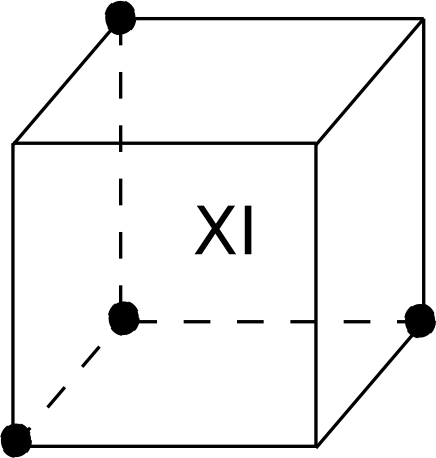
\includegraphics[width=2cm]{pyramid-0.png} &
 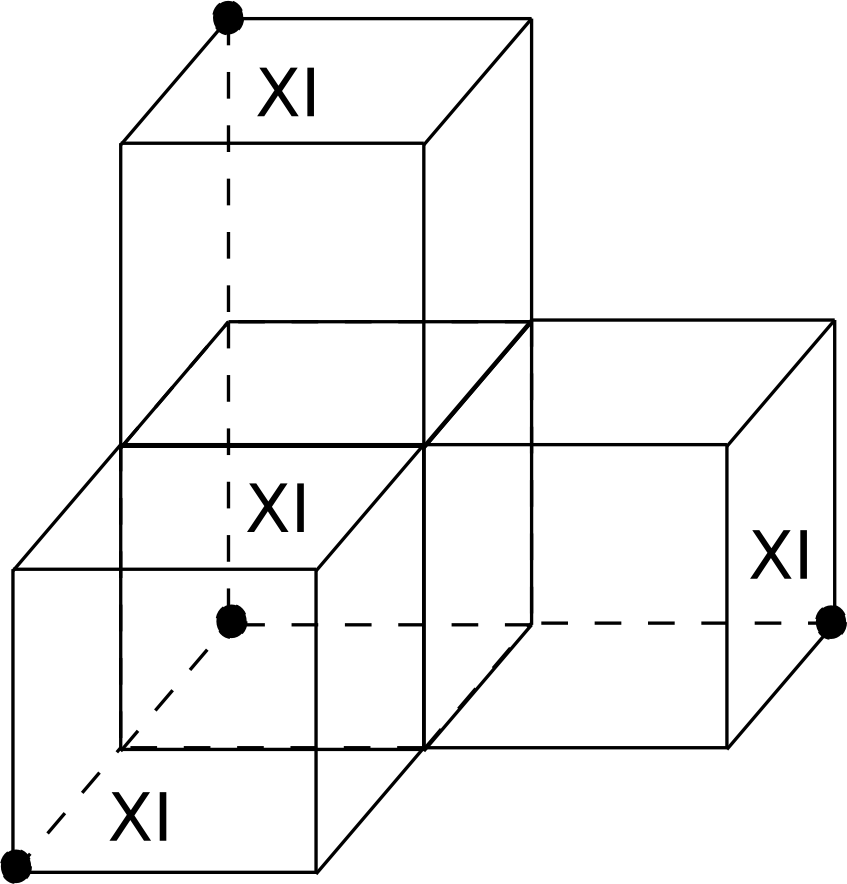
\includegraphics[width=3cm]{pyramid-1.png}
\end{tabular}
\caption{Isolating a topological excitation. The cubes are in the dual lattice; each vertex represents an elementary cube in the primary lattice.}
\label{fig:pyramid}
\end{figure}



We show that the cubic code model can be used as a quantum memory at nonzero temperatures in the following sense. We develop a well-defined read-out procedure (decoder) with which a ground state maintains coherence for time proportional to $L^{c \beta}$ where $L$ is a linear system size and $\beta$ is an inverse temperature. This statement is valid only if $L \le e^{c' \beta}$. Roughly speaking, this is because of a large entropic contribution from the point-like excitations. For small system size, the entropic contribution is small. At an optimal system size, the memory time is $e^{c c' \beta^2}$. A natural question is then whether we could remove all such point-like excitations. We answer this question negatively: There must be an isolated point-like excitation in any topologically ordered three-dimensional quantum code model if it is translationally invariant. The proof is based on a formalism using translation group algebras and free resolutions of finitely generated modules.


\section{Summary of chapters}


In Chapter~\ref{chap:additive-codes}, we explain a general structure of a class of quantum error correcting codes, called additive or stabilizer codes. It is emphasized that the additive code is described by a binary vector space. A simple counting of vector space dimensions yields {\em cleaning lemma}. It states that the number of independent logical operators on complementary regions add up to the total number of independent logical operators of the code. Combining the geometric locality of two-dimensional Hamiltonian with the cleaning lemma, we prove a trade-off theorem about the support of the logical operators. In particular, this implies that only string operators act on the ground-state subspace in two-dimensional quantum codes. 
The content is published in \cite{HaahPreskill2012tradeoff}.


In Chapter~\ref{chap:alg-theory}, we develop a formulation of translationally invariant quantum codes. We observe that they have a succinct description by a matrix $\sigma$ over the translation group algebra which is commutative. The local indistinguishability is interpreted as a vanishing homology of a complex defined by $\sigma$. Local unitary transformations and coarse-graining are described by simple matrix operations. The ground-state degeneracy is approximated as the number of points on an algebraic variety defined by $\sigma$ over finite fields. Fractal operators and point-like excitations are defined, and the set of all point-like excitations modulo locally created ones is identified with a specific module.
The content is published in \cite{Haah2012PauliModule}.


In Chapter~\ref{chap:lowD-codes}, we use the formalism of Chapter~\ref{chap:alg-theory} to derive consequences of physical dimensionality. The translation invariance is imposed. One-dimensional codes are classified completely. Up to local unitary transformations, any code decomposes into finitely many 1D Ising models. In two dimensions, we prove that there are finitely many types of topological excitations and they are all appear as end points of string operators.
In three dimensions, we prove that there must exist a point-like topological excitation. If the ground-state degeneracy is constant independent of system size, we show that the point-like topological excitations are attached to string operators. Examples are presented for which our formalism is useful.
The content is published in \cite{Haah2012PauliModule}.


In Chapter~\ref{chap:cubic-code}, we explain how the cubic code is found. It is a result of an exhaustive but systematic search. We prove important properties of the cubic code such as the topological order, ground-state degeneracy, and the absence of string operators. The cubic code's thermal partition function is computed to show that the free energy density is smooth in the thermodynamic limit as a function of temperature. An entanglement renormalization group flow is presented. We find that the cubic code (A) bifurcates into itself (A) and another model B. The new model B shares all important properties of A, but is different from A. Under a further real-space renormalization, B bifurcates into two copies of itself. 
A part of the content in this chapter is published in \cite{Haah2011Local}. Our presentation in this thesis is more succinct than that in the published paper, due to algebraic methods of Chapter~\ref{chap:alg-theory} developed more recently.


In Chapter~\ref{chap:consq-no-strings}, we prove theorems implied by the absence of string operators. The theorems quantifies the energy landscape of the Hamiltonian on the ``land'' of energy eigenstates. Two states are considered to be ``close'' in the land if one state can be transformed to the other by a single spin operator; if it is necessary to apply many spin operators, the two states are considered to be far apart in the land. On this land of states, imagine hills whose height is given by the energy of the state. The landscape of this land is analogous to a potential energy barrier in a quantum mechanical tunneling problem. We define the {\em energy barrier} to be the height of the lowest hill on any path in the land connecting two states. We prove that between two ground states there exists an energy barrier larger than the logarithm of the system size $L$, and the distance in the land is at least $L^\gamma$ with $\gamma > 1$. A closely related statement reads that between a ground state and a state where a topological excitation is isolated from others by distance $R$, there exists an energy barrier $\ge \log R$, and the distance in the land is $\ge R^\gamma$ with $\gamma >1$.
The content is published in \cite{BravyiHaah2011Energy}.


In Chapter~\ref{chap:RG-decoder}, we design a decoding algorithm. Any physical memory cannot be pristine after contact with an error source. In order to retrieve correct information for the next step of processing, one needs to map the affected state to the ground state. For a ferromagnet this decoding process amounts to measuring average magnetization. For quantum codes, the first step is to detect errors. This is done by measuring the terms in the commuting Hamiltonian. The next step is to guess probable types and locations of errors, which we specifically call ``decoding algorithm.'' Once error locations and types are identified, the final step is to undo the errors. A good decoder should map corrupt states to its original pristine state with high probability. Our algorithm uses a hierarchy of subroutines which borrows ideas from renormalization group. It is widely applicable and is efficient with running time $O(V\log V)$ where $V$ is the volume of the system. Moreover, we prove that there is a positive critical error probability, called a threshold, below which the decoding algorithm succeeds asymptotically perfectly in the limit of large system size. Our decoder is the first decoder that admits an efficient implementation and a rigorous threshold theorem.
The content is published in \cite{BravyiHaah2011Memory}.


In Chapter~\ref{chap:q-mem}, we directly assess the performance of the cubic code as a robust quantum memory at nonzero temperature. One ingredient is to show that the decoding algorithm of Chapter~\ref{chap:RG-decoder} corrects errors of low energy barriers. Here, the energy barrier of an error is defined in the same way as above --- the height of lowest hill in the energy landscape on any path connecting a ground state and the state affected by the error. Another ingredient is an analysis of Markovian master equation exploiting the fact that there exists a good decoder $\Phi_{ec}$, a trace preserving completely positive quantum operation. An analytic bound on the trace distance between the initial state $\rho(0)$ and the error-corrected time-evolved state $\Phi_{ec}(\rho(t))$ is given as
\[
\| \rho(0) - \Phi_{ec}(\rho(t)) \| \le t \frac{(1+e^{-\beta})^V}{V^{\beta}}
\]
where $V$ is the system volume and $\beta$ is the inverse temperature, neglecting all unimportant constant coefficients. If $V \le e^\beta$, the bound says the fidelity of error-corrected $\Phi_{ec}(\rho(t))$ remains close to $\rho(0)$ until $t \sim V^\beta$. We complement the bound with a numerical simulation, which suggests that our bound is optimal up to constant coefficients.
The content is published in \cite{BravyiHaah2011Memory}.
